\documentclass[tikz,border=8pt]{standalone}
% Shared look for every TikZ diagram. Load with % Shared look for every TikZ diagram. Load with % Shared look for every TikZ diagram. Load with \input{../../tools/tikz-style.tex}
\usepackage[T1]{fontenc}
\usepackage{lmodern}
\renewcommand{\sfdefault}{lmr}  % diagrams use the same serif as the text
\usetikzlibrary{arrows.meta, positioning, shapes.geometric, calc, fit, backgrounds}
\definecolor{cblue}{HTML}{4C78A8}
\definecolor{corange}{HTML}{F58518}
\definecolor{cgreen}{HTML}{54A24B}
\definecolor{cred}{HTML}{E45756}
\definecolor{cpurple}{HTML}{B279A2}
\definecolor{cgrey}{HTML}{6B6B6B}
\tikzset{
  every picture/.style={font=\sffamily, line width=1.2pt},
  box/.style={draw=#1, fill=#1!12, rounded corners=4pt, align=center, inner sep=7pt, minimum height=1.1cm},
  box/.default=cgrey,
  arrow/.style={-{Stealth[length=3mm]}, draw=cgrey, line width=1.4pt},
  title/.style={font=\sffamily\bfseries\Large},
  note/.style={font=\sffamily\small, text=cgrey, align=center},
}
\AtBeginDocument{\hyphenpenalty=10000 \exhyphenpenalty=10000}

\usepackage[T1]{fontenc}
\usepackage{lmodern}
\renewcommand{\sfdefault}{lmr}  % diagrams use the same serif as the text
\usetikzlibrary{arrows.meta, positioning, shapes.geometric, calc, fit, backgrounds}
\definecolor{cblue}{HTML}{4C78A8}
\definecolor{corange}{HTML}{F58518}
\definecolor{cgreen}{HTML}{54A24B}
\definecolor{cred}{HTML}{E45756}
\definecolor{cpurple}{HTML}{B279A2}
\definecolor{cgrey}{HTML}{6B6B6B}
\tikzset{
  every picture/.style={font=\sffamily, line width=1.2pt},
  box/.style={draw=#1, fill=#1!12, rounded corners=4pt, align=center, inner sep=7pt, minimum height=1.1cm},
  box/.default=cgrey,
  arrow/.style={-{Stealth[length=3mm]}, draw=cgrey, line width=1.4pt},
  title/.style={font=\sffamily\bfseries\Large},
  note/.style={font=\sffamily\small, text=cgrey, align=center},
}
\AtBeginDocument{\hyphenpenalty=10000 \exhyphenpenalty=10000}

\usepackage[T1]{fontenc}
\usepackage{lmodern}
\renewcommand{\sfdefault}{lmr}  % diagrams use the same serif as the text
\usetikzlibrary{arrows.meta, positioning, shapes.geometric, calc, fit, backgrounds}
\definecolor{cblue}{HTML}{4C78A8}
\definecolor{corange}{HTML}{F58518}
\definecolor{cgreen}{HTML}{54A24B}
\definecolor{cred}{HTML}{E45756}
\definecolor{cpurple}{HTML}{B279A2}
\definecolor{cgrey}{HTML}{6B6B6B}
\tikzset{
  every picture/.style={font=\sffamily, line width=1.2pt},
  box/.style={draw=#1, fill=#1!12, rounded corners=4pt, align=center, inner sep=7pt, minimum height=1.1cm},
  box/.default=cgrey,
  arrow/.style={-{Stealth[length=3mm]}, draw=cgrey, line width=1.4pt},
  title/.style={font=\sffamily\bfseries\Large},
  note/.style={font=\sffamily\small, text=cgrey, align=center},
}
\AtBeginDocument{\hyphenpenalty=10000 \exhyphenpenalty=10000}

\begin{document}
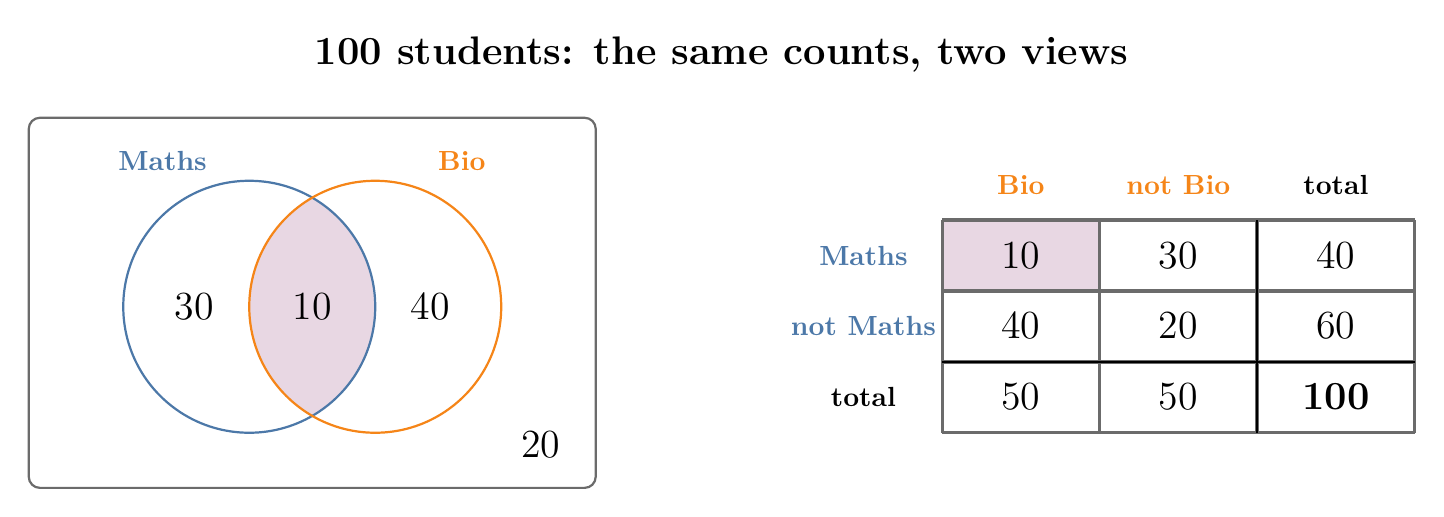
\begin{tikzpicture}[x=1cm, y=1cm]
  \node[title] at (5.2,3.2) {100 students: the same counts, two views};
  % Venn
  \draw[thick, rounded corners, draw=cgrey] (-3.6,-2.3) rectangle (3.6,2.4);
  \begin{scope}
    \clip (-0.8,0) circle (1.6);
    \fill[cpurple!30] (0.8,0) circle (1.6);
  \end{scope}
  \draw[thick, cblue] (-0.8,0) circle (1.6);
  \draw[thick, corange] (0.8,0) circle (1.6);
  \node[text=cblue, font=\sffamily\bfseries] at (-1.9,1.85) {Maths};
  \node[text=corange, font=\sffamily\bfseries] at (1.9,1.85) {Bio};
  \node[font=\sffamily\Large] at (-1.5,0) {30};
  \node[font=\sffamily\Large] at (0,0) {10};
  \node[font=\sffamily\Large] at (1.5,0) {40};
  \node[font=\sffamily\Large] at (2.9,-1.75) {20};
  % table
  \begin{scope}[shift={(6.0,-1.6)}]
    \def\w{2.0} \def\h{0.9}
    \node[font=\sffamily\bfseries] at (1.5*\w,4*\h+0.35) {};
    \node[font=\sffamily\bfseries, text=corange] at (1.5*\w,3.5*\h) {Bio};
    \node[font=\sffamily\bfseries, text=corange] at (2.5*\w,3.5*\h) {not Bio};
    \node[font=\sffamily\bfseries] at (3.5*\w,3.5*\h) {total};
    \node[font=\sffamily\bfseries, text=cblue] at (0.5*\w,2.5*\h) {Maths};
    \node[font=\sffamily\bfseries, text=cblue] at (0.5*\w,1.5*\h) {not Maths};
    \node[font=\sffamily\bfseries] at (0.5*\w,0.5*\h) {total};
    \fill[cpurple!30] (\w,2*\h) rectangle (2*\w,3*\h);
    \draw[cgrey] (\w,0) grid[xstep=\w, ystep=\h] (4*\w,3*\h);
    \draw[thick] (\w,\h) -- (4*\w,\h);
    \draw[thick] (3*\w,0) -- (3*\w,3*\h);
    \node[font=\sffamily\Large] at (1.5*\w,2.5*\h) {10};
    \node[font=\sffamily\Large] at (2.5*\w,2.5*\h) {30};
    \node[font=\sffamily\Large] at (1.5*\w,1.5*\h) {40};
    \node[font=\sffamily\Large] at (2.5*\w,1.5*\h) {20};
    \node[font=\sffamily\Large] at (3.5*\w,2.5*\h) {40};
    \node[font=\sffamily\Large] at (3.5*\w,1.5*\h) {60};
    \node[font=\sffamily\Large] at (1.5*\w,0.5*\h) {50};
    \node[font=\sffamily\Large] at (2.5*\w,0.5*\h) {50};
    \node[font=\sffamily\Large\bfseries] at (3.5*\w,0.5*\h) {100};
  \end{scope}
\end{tikzpicture}
\end{document}
